% Шаблон (версия от 15.02.2016) предназначен 
% для использования студентами каф. ПМиИ СамГТУ 
% при оформлении отчетов по лабораторным работам. 
% Для настройки пакета listigs использовался материал 
% статьи Михаила Конника aka virens
% <http://mydebianblog.blogspot.ru/2012/12/latex.html>
% Copyright (c) 2016 by Mikhail Saushkin (msaushkin@gmail.com) 
% All rights reserved except the rights granted by the
% Creative Commons Attribution 4.0 International Licence
% <https://creativecommons.org/licenses/by/4.0/>
% Свежая версия шаблона здесь <https://www.overleaf.com/read/sqvxbnhgxxdm>
\documentclass[14pt,a4paper,report]{ncc}
\usepackage[a4paper, mag=1000, left=2.5cm, right=1cm, top=2cm, bottom=2cm, headsep=0.7cm, footskip=1cm]{geometry}
\usepackage[utf8]{inputenc}
\usepackage[english,russian]{babel}
\usepackage{indentfirst}
\usepackage[dvipsnames]{xcolor}
\usepackage[colorlinks]{hyperref}
\usepackage{listings} 
\usepackage{caption}
\usepackage{amssymb}
\usepackage{tcolorbox}
\DeclareCaptionFont{white}{\color{white}} %% это сделает текст заголовка белым
%% код ниже нарисует серую рамочку вокруг заголовка кода.
\usepackage{color} %% это для отображения цвета в коде
\DeclareCaptionFormat{listing}{\colorbox{gray}{\parbox{\textwidth}{#1#2#3}}}
\captionsetup[lstlisting]{format=listing,labelfont=white,textfont=white}
\lstset{% Собственно настройки вида листинга
inputencoding=utf8, extendedchars=\true, keepspaces = true, % поддержка кириллицы и пробелов в комментариях
language=C++,            % выбор языка для подсветки (здесь это Pascal)
numberstyle =\tiny
basicstyle=\small\sffamily, % размер и начертание шрифта для подсветки кода
keywordstyle =\color{ForestGreen},
numbers=left,               % где поставить нумерацию строк (слева\справа)
numberstyle=\tiny,          % размер шрифта для номеров строк
stepnumber=1,               % размер шага между двумя номерами строк
numbersep=5pt,              % как далеко отстоят номера строк от подсвечиваемого кода
backgroundcolor=\color{white}, % цвет фона подсветки - используем \usepackage{color}
showspaces=false,           % показывать или нет пробелы специальными отступами
showstringspaces=false,     % показывать или нет пробелы в строках
showtabs=false,             % показывать или нет табуляцию в строках
frame=single,               % рисовать рамку вокруг кода
tabsize=2,                  % размер табуляции по умолчанию равен 2 пробелам
captionpos=t,               % позиция заголовка вверху [t] или внизу [b] 
breaklines=true,            % автоматически переносить строки (да\нет)
breakatwhitespace=false,    % переносить строки только если есть пробел
escapeinside={\%*}{*)}      % если нужно добавить комментарии в коде
}

\begin{document}
% Переоформление некоторых стандартных названий
%\renewcommand{\chaptername}{Лабораторная работа}
\def\contentsname{Содержание}

% Оформление титульного листа
\begin{titlepage}
\begin{center}
\textsc{ФГОУ ВО Уральский Федеральный Университет \\ имени первого Президента России Б.Н.Ельцина\\[5mm]
Физико-технологический институт\\[2mm]
Кафедра теоретической физики и прикладной математики}

\vfill

\textbf{ОТЧЁТ ПО ЛАБОРАТОРНОЙ РАБОТЕ №1\\[3mm]
«Симуляция двумерной системы частиц взаимодействующих через потенциал Леннарда-Джонса с учетом периодических граничных условий»\\[6mm]
}
\end{center}

\hfill
\begin{minipage}{.5\textwidth}
Студент:\\[2mm] 
Вялова С.А.\\
группа: ФтМ-170403 \\[5mm]

Преподаватель:\\[2mm] 
д.ф.-м.н., профессор\\
Мазуренко Владимир Владимирович\\[5mm]

Консультант:\\[2mm] 
н.с.\\
Сотников Олег Михайлович\\

\end{minipage}%
\vfill
\begin{center}
\today  \\
%\theyear\, г.
 Екатеринбург.
\end{center}
\end{titlepage}

% Содержание
\tableofcontents
\newpage
\chapter{Моделирование двумерной системы частиц, взаимодействующих через потенциал Леннарда-Джонса}
\section{Цель работы}


Разработка программы для симуляции молекулярной динамики двумерной системы частиц, взаимодействующих через потенциал Леннарда-Джонса с учётом периодический граничных условий, а также применение алгоритма Верле для решения уравнения движения. Начальные значения координат и скоростей частиц выбираются так, чтобы выполнялось условие нулевого импульса системы.

\
Реализуются следующие пункты:

\begin{itemize}
\item Возможность задания произвольного числа частиц;
\item расчет кинетической, потенциальной и полной энергии;
\item определение и контроль температуры системы;
\item визуализация всей системы  и траектории отдельной частицы;
\item расчет среднеквадратичного смещения и автокорреляционной функции скорости.
\end{itemize}
\newpage\section{Теоретическая часть }
\subsection{Потенциал Леннарда-Джонса}
%text
Потенциал Леннарда-Джонса представляет собой простую модель парного взаимодействия неполярных молекул, описывающая зависимость энергии взаимодействия двух частиц от расстояния между ними.
Потенциал был предложен Леннардом-Джонсом первоначально для исследования термодинамических свойств инертных газов. Наиболее часто используется так называемый (6-12)-потенциал Леннарда-Джонса, записанный в форме 
\
\begin{equation}
 U = 4 \cdot \varepsilon \cdot [(\sigma/r)^{12} - (\sigma/r)^{6}  ] ,
 \end{equation} 
где $\varepsilon$ - глубина потенциальной ямы, $\sigma$ - значение расстояния между частицами, при котором потенциал равен нулю. Шестая степень убывания отвечает электростатическому диполь-дипольному и дисперсионному притяжению; двенадцатая степень убывания потенциала моделирует достаточно жесткое отталкивание и выбрана из соображений математического удобства.
\

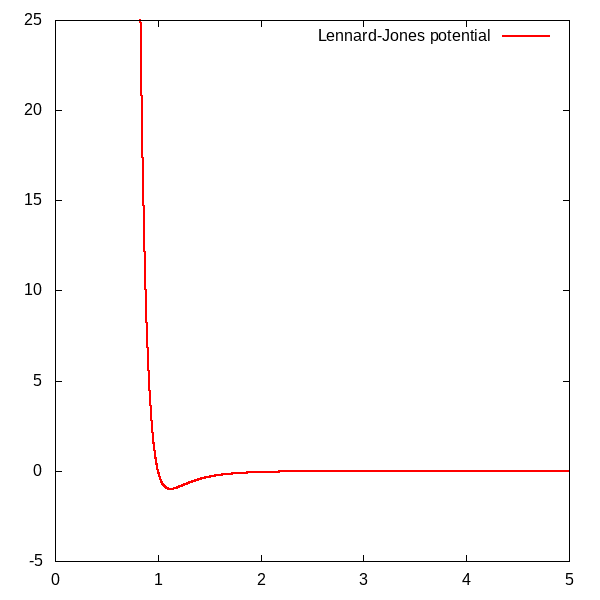
\includegraphics[scale=0.8]{plot_lgpotential}
%\caption{Зависимость температуры системы от шага по времени.}


\subsection{Описание вычислительного метода}
%text
Для моделирования системы, состоящей из N взаимодействующих частиц необходимо численно решить классические уравнения движения системы
\begin{equation}
m_{i}\dot{\vec{v_i}}=F_{i}(t, \vec{x_1}, ... ,  \vec{x_N}, \vec{v_1}, ... , \vec{v_N})
\end{equation}
\begin{equation}
\dot{\vec{x_i}}=\vec{v_i}.
\end{equation}
Сила, действующая на i-ю частицу, может быть найдена как градиент потенциала: 
\begin{equation}
\vec{F}_i= -\vec{\nabla}U(\vec{r})
\end{equation} 
Чтобы начать моделировать двумерную систему взаимодействующих частиц, необходимо задать все координаты частиц, равномерно расположив их относительно друг друга, а также их скорости. Каждая пара частиц взаимодействует через потенциал Леннарда-Джонса.
\begin{equation}
\vec{r}_{n+1} = \vec{r}_{n} + \vec{v}_{n}\cdot{dt}
\end{equation}
\begin{equation}
\vec{v}_{n+1}=\vec{v}_{n}+\frac{1}{2} \cdot (\vec{a}_n+\vec{a}_{n+1})
\end{equation}
Ускорения определяем из потенциала Леннарда-Джонса:
\begin{equation}
\vec{F}_i= -\vec{\nabla}U(\vec{r}) = m_i \vec{a}_i
\end{equation}
Подставляя выражение для потенциала Леннарда-Джонса (1.1) в выражение для силы (1.7), действующей на каждую частицу со стороны системы, получаем ускорение i-й частицы:
\begin{equation}
\vec{a}_i=4  \varepsilon \cdot  \sum\limits_{i=j}^N \sum\limits_{j \neq i}^N{\frac{\vec{r}_{ij}}{m_i | \vec{r}_{ij}|^2}  [2  (\sigma/\vec{r}_{ij})^{12}-(\sigma/\vec{r}_{ij})^6]}
\end{equation}
Из полученных данных возможно вычислить кинетическую (1.9) и потенциальную (1.10) энергии системы:
\begin{equation}
E_{kinetic} = \sum\limits_{i=1}^N{\frac{m_i {\vec{v}}^2_i}{2}}
\end{equation}
\begin{equation}
E_{potential}=4 \varepsilon \sum\limits_{i=1}^N \sum\limits_{s=i+1}^N{ [(\sigma/\vec{r}_{is})^{12} - (\sigma/\vec{r}_{is})^{6}  ]}
\end{equation}
Полная энергия системы (1.11) вычисляется как сумма кинетических и потенциальных энергий всех частиц в системе.
\begin{equation}
E_{total}=E_{kinetic}+E_{potential}
\end{equation}
Важным критерием является неизменность полной энергии системы на каждом шаге.
\ 
Используемый для решение поставленной задачи вычислительный алгоритм требует нулевого суммарного импульса системы частиц.
Требование нулевого суммарного импульса системы удовлетворяется за счёт перенормировки заданных начальных скоростей следующим образом:
\begin{equation}
\vec{v}_{{i} \ new} = \vec{v}_i - {\frac{1}{N}}\sum\limits_{i=1}^N \vec{v}_i
\end{equation}

Также необходимо было реализовать контроль температуры, суть которого заключается в том, чтобы по прошествии заданного числа итераций, когда система окажется в равновесии с некоторой температурой $T_{current}$ , на систему воздействовал мгновенный импульс, задача которого - перевести систему в равновесие с некоторой заданной температурой $T_{desired}$. 
\ 

Осуществляется это следующим образом: на заданном шаге все скорости частиц в системе умножаются на масштабирующий коэффициент $k=\sqrt{\frac{T_{desired}}{T_{current}}}$. Далее продолжается моделирование системы, которая релаксировала к состоянию с заданной температурой.
\newpage\section{Практическая часть}
\subsection{Описание функционала разработанной программы}
%text
Для выполнения поставленной задачи выбран язык программирования C++. Входные данные задаются пользователем с клавиатуры. Программе необходимо передать значение общего числа частиц в системе, значение постоянной решётки, шаг по времени, а также число шагов по времени, значения параметров модели $\sigma$ и $\varepsilon$.
\

Далее программа генерирует исходные координаты частиц в системе в виде сетки в пределах постоянной решётки, произвольные значения начальных скоростей частиц в указанных линейных диапазонах, впоследствии пересчитывая скорости в соответствии с требованием нулевого суммарного имульса системы. Вычисляются ускорения и скорости для следующего шага по времени, координаты частиц в системе с учётом периодических граничных условий, и далее, в цикле по шагу по времени, программа вычисляет ускорения для новых положений частиц, скорости, кинетическую, потенциальную энергии системы, а также координаты для следующего, (n+1)-го шага по времени.
\

\begin{figure}[h]
\center{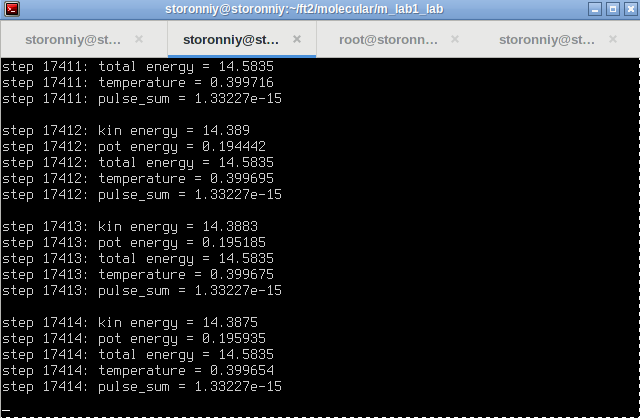
\includegraphics[width=1\linewidth]{program}}
\caption{Демонстрация выполняющейся программы.}
\label{ris:image}
\end{figure}
Запуск программы осуществляется из коммандной оболочки bash (рисунок 1.1). В ходе выполнения программа для каждого шага по времени выводит в терминал значения кинетической, потенциальной и полной энергии системы, температуру системы, а также значение суммарного импульса для контроля, а также в выходные файлы на каждом шаге записываются координаты частиц, кинетическая, потенциальная и полная энергии системы, температура системы, значение функции среднеквадратического смещения частиц и автокорреляционной функции скорости. По записанным данным могут быть построены графики зависимостей данных величин от шага по времени.
\



\
\subsection{Визуализация всей системы и траектории отдельной частицы}
При моделировании системы были использованы следующие входные данные:
\begin{itemize}
\item значение параметра $\sigma$=2.74;
\item значение параметра $\varepsilon$=0.0031;
\item линейный размер системы L=40;
\item число частиц N=36;
\item шаг по времени dt=0.0001;
\item число шагов по времени NSTEP=1000000;
\item диапазон начальных скоростей [-1; 1];
\item шаг начала контроля температуры N=100000;
\item конечная температура T=0.4.
\end{itemize}
\

Заданное число частиц системы располагается в виде равномерной квадратной сетки внутри ячейки со стороной, равной постоянной решетки. Функционал разработанной программы для моделирования данной системы частиц предполагает на выходе файл, содержащий набор всех координат частиц на каждом шаге моделирования, поэтому эволюция положения частиц системы была визуализирована с использованием пакета Gnuplot в виде gif-изображения. Положения всех частиц системы, находящейся в исходном состоянии и на некотором шаге в ходе моделирования, представлены на рисунке 1.2(а) и рисунке 1.2(б) соответственно.


\begin{figure}[!h]
\begin{minipage}[!h]{0.5\linewidth}
\center{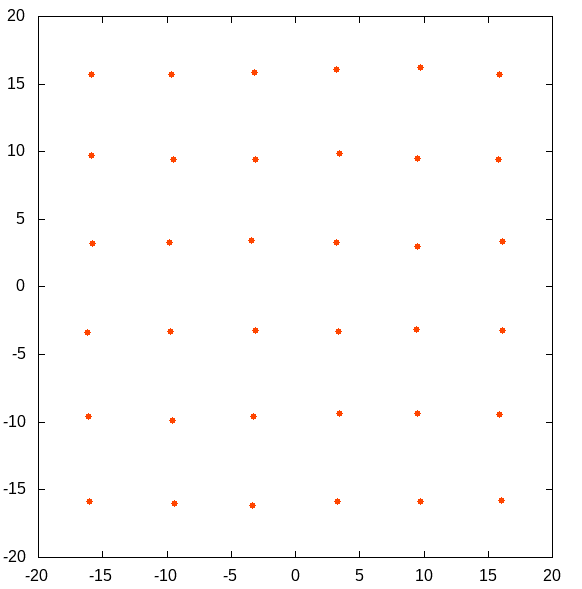
\includegraphics[width=1\linewidth]{initial} \\ а)}
\end{minipage}
\hfill
\begin{minipage}[!h]{0.5\linewidth}
\center{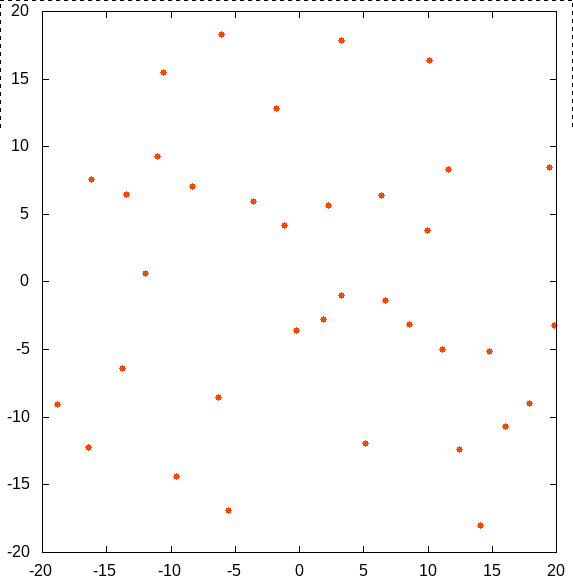
\includegraphics[width=1\linewidth]{system} \\ б)}
\end{minipage}
\caption{Положение частиц в системе а) в исходном состоянии; б) в ходе моделирования.}
\end{figure}
 \
Трактория отдельной частицы представлена на рисунке 1.3. Изменение направления импульса частицы означает столкновение данной частицы с другими частицами системы. Периодические граничные условия, как видно, заставляют частицу, выходящую за границы рассматриваемой области, "появляться" с противоположной стороны рассматриваемой области.
\begin{figure}[!h]
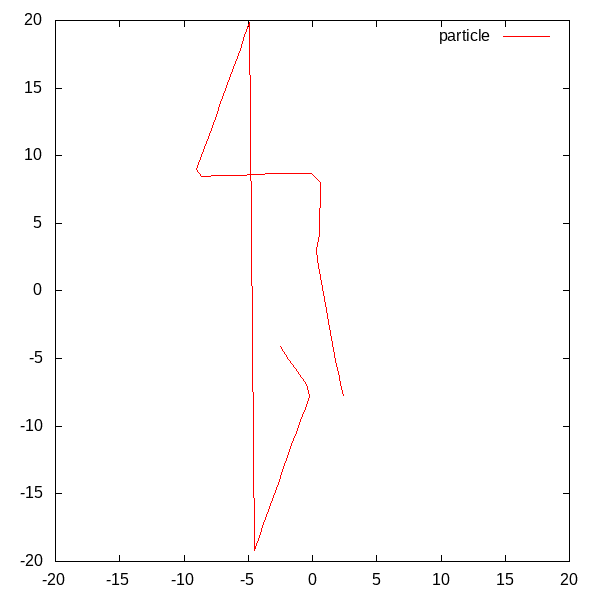
\includegraphics[scale=0.8]{particle}
\caption{Траектория отдельной частицы.}
\end{figure}
 \
 \subsection{Результаты моделирования}
В ходе моделирования были получены графики зависимости кинетической, потенциальной и полной энергии системы от шага по времени (рисунок 1.4), а также температуры системы и средней температуры системы от шага по времени (рисунок 1.5).
\

\begin{figure}[!h]
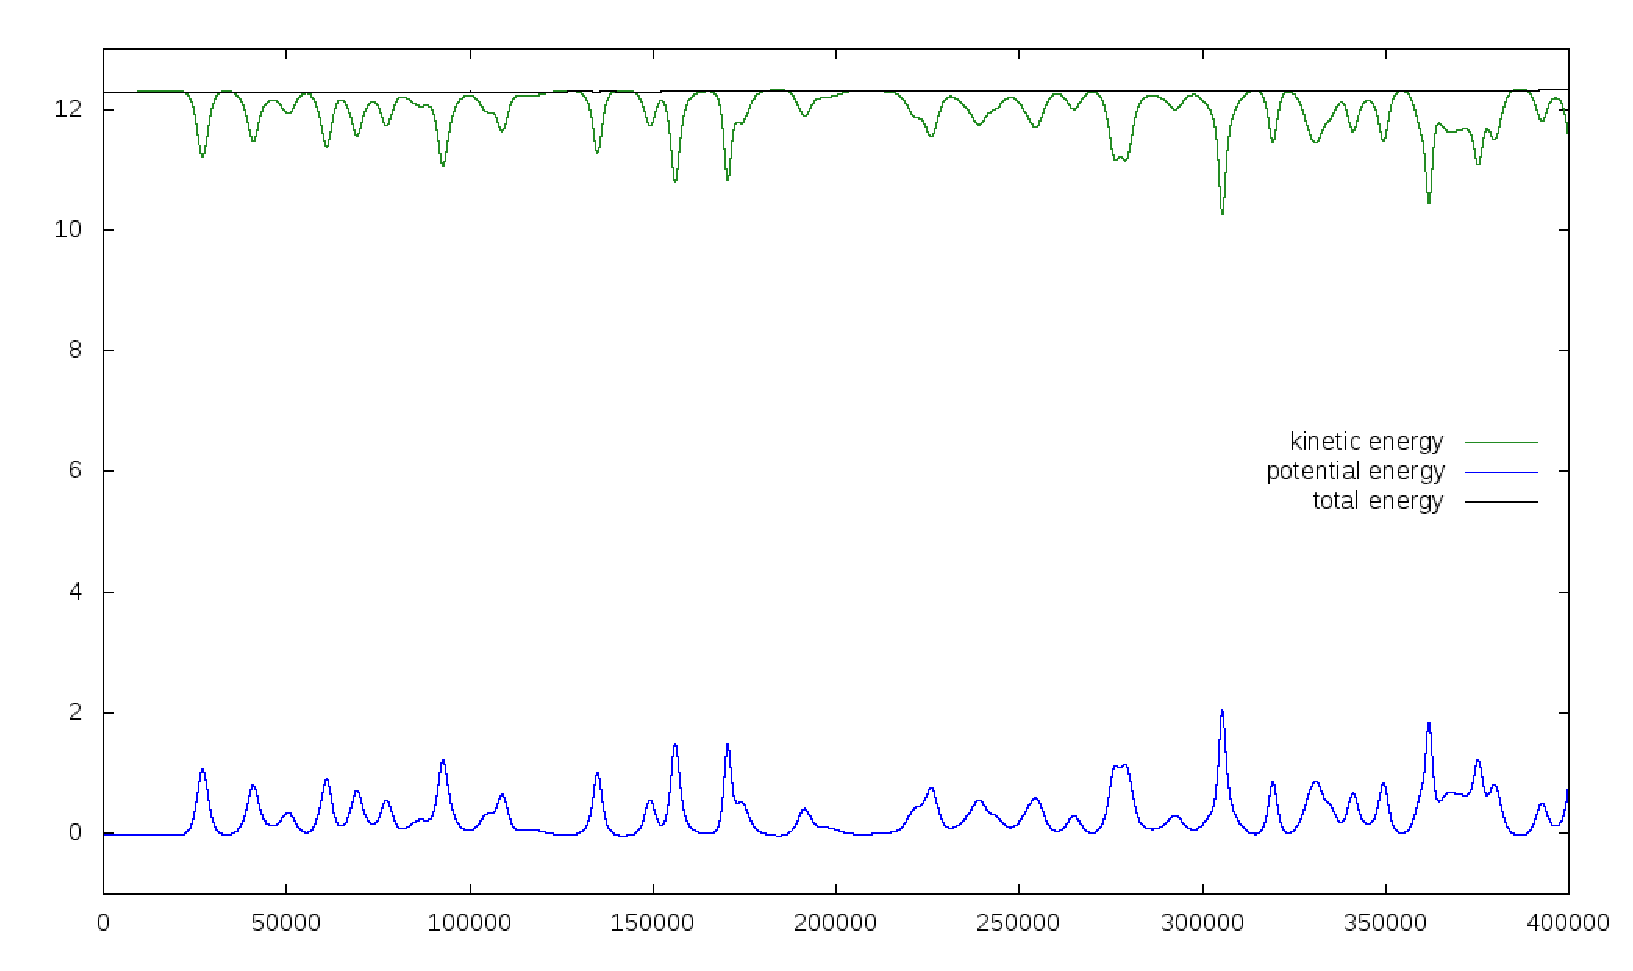
\includegraphics[scale=0.6]{energy400}
\caption{Зависимость кинетической (зеленый), потенциальной (синий) и полной (черный) энергии системы от шага по времени.}
\end{figure}
График зависимости потенциальной, кинетической и полной энергии системы от шага моделирования указывает на то, что закон cохранения полной энергии в системе выполняется, то есть полная энергия системы не изменяется в ходе эволюции системы.
\begin{figure}[h!]
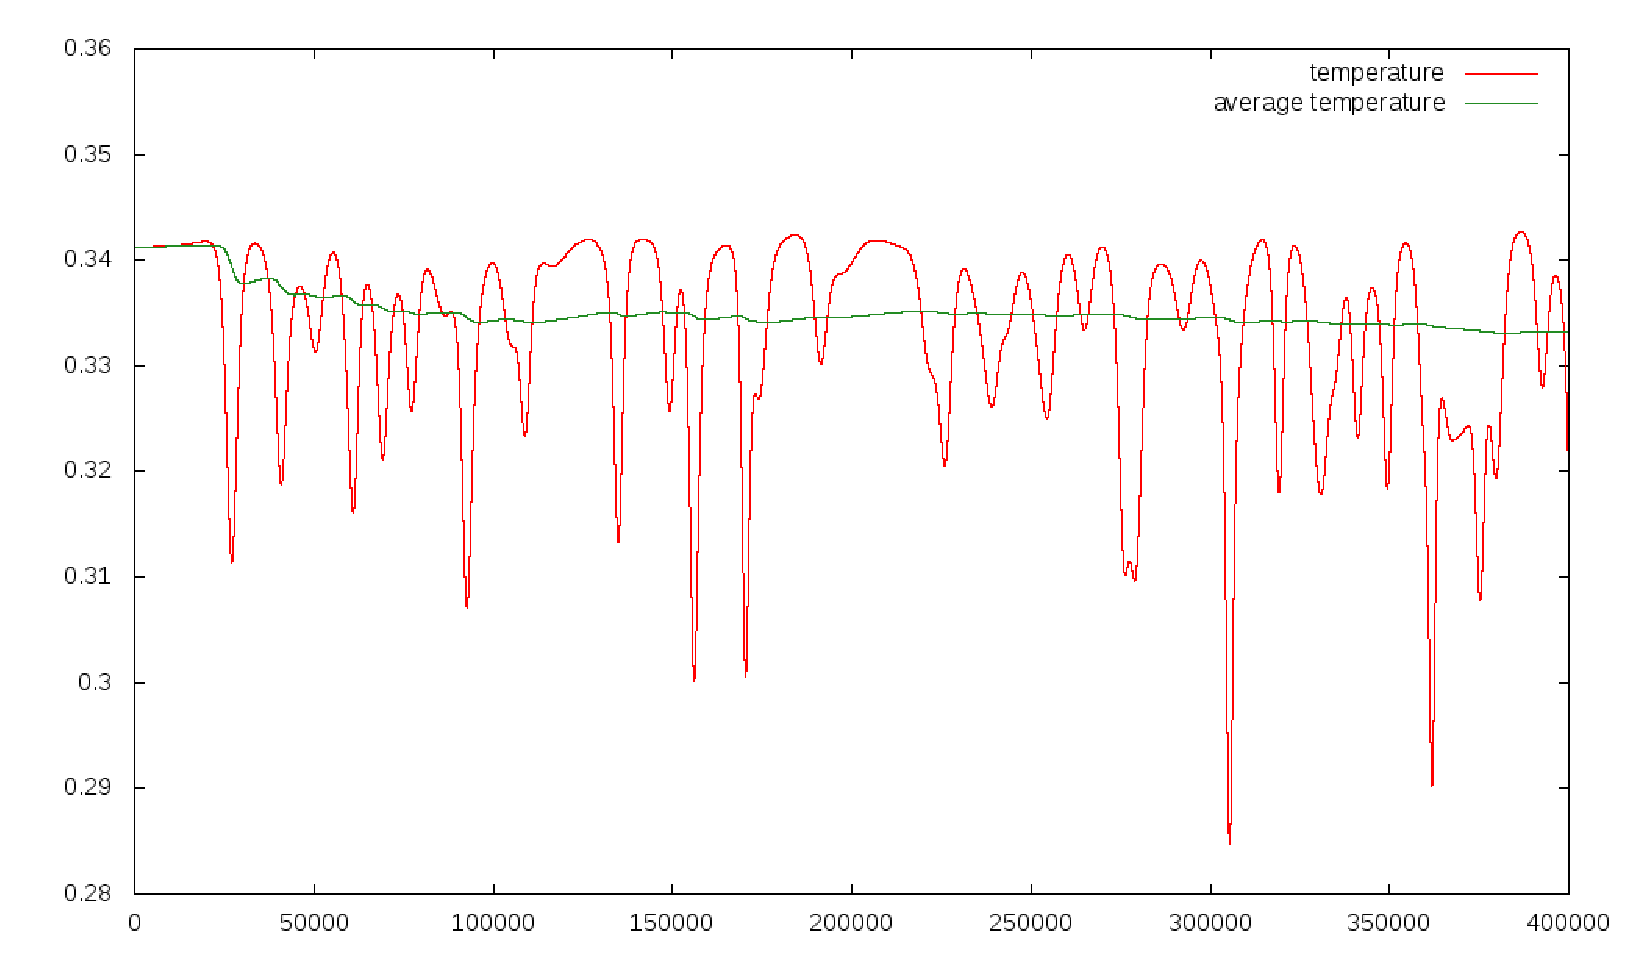
\includegraphics[scale=0.6]{temp400}
\caption{Зависимость средней (зеленый) и мгновенной (красный) температуры системы от шага по времени.}
\end{figure}


Требование нулевого суммарного импульса системы, как видно из графика 1.6, выполняется.
\

Также были построены графики среднеквадратического смещения (рис 1.7) и автоколлеляционной функции скорости (рис. 1.8). Из графика 1.8 видно, что первые 20000 шагов частицы движутся почти без столкновений, это соответствует квадратичной зависимости среднеквадратического смещения (рис. 1.7). Далее следует скачок потенциальной энергии системы с изменением характера движения с баллистического на диффузионный, что отражается резким спадом автокорреляционной функции скорости и линейной частью среднеквадратического смещения.
\
\begin{figure}[h!]
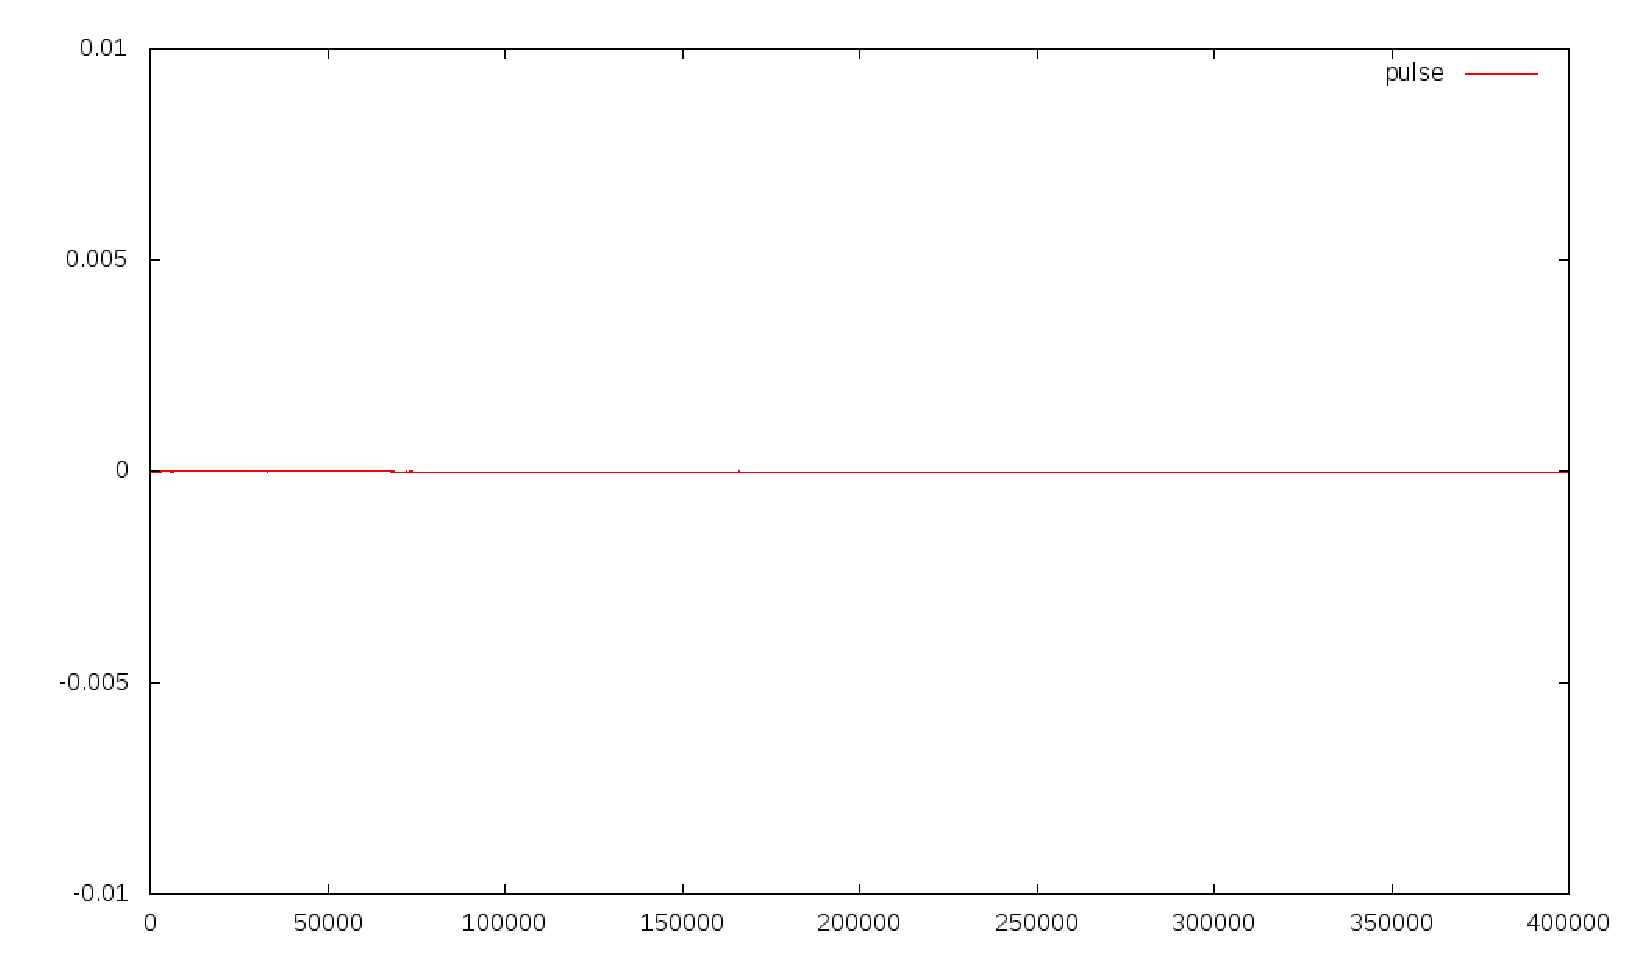
\includegraphics[scale=0.6]{pulse400eps}
\caption{Зависимость суммарного импульса системы от шага по времени.}
\end{figure}

\begin{figure}[!h]
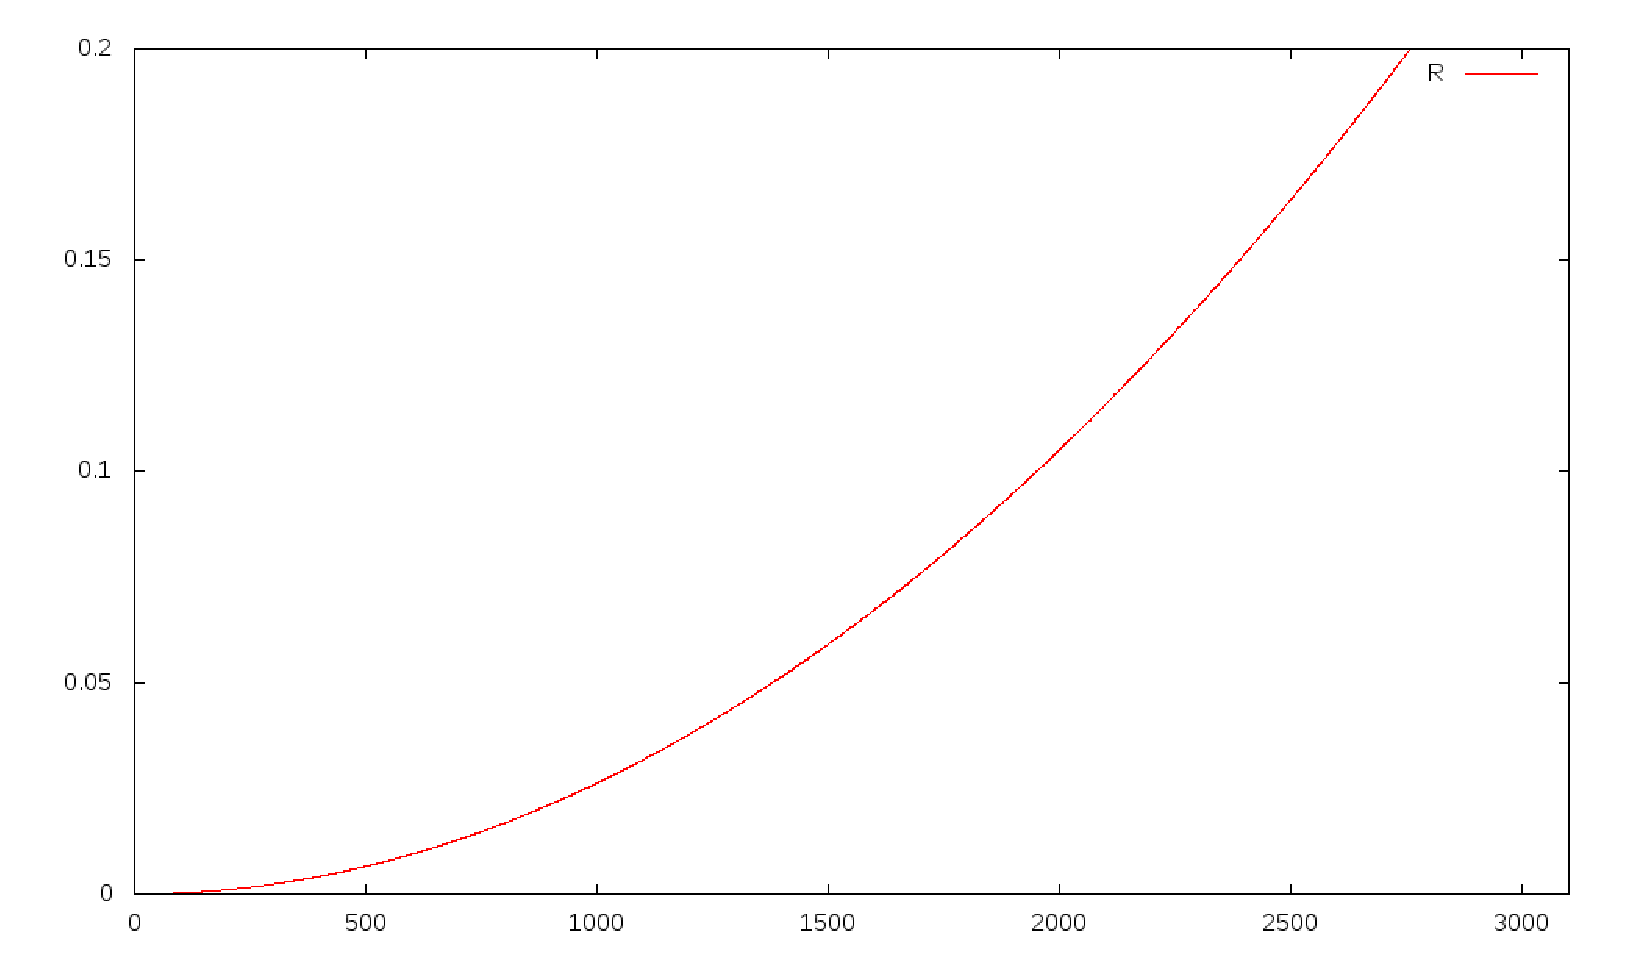
\includegraphics[scale=0.6]{R380eps}
\caption{Зависимость среднеквадратического смещения частиц системы от шага по времени.}
\end{figure}
\begin{figure}[!h]
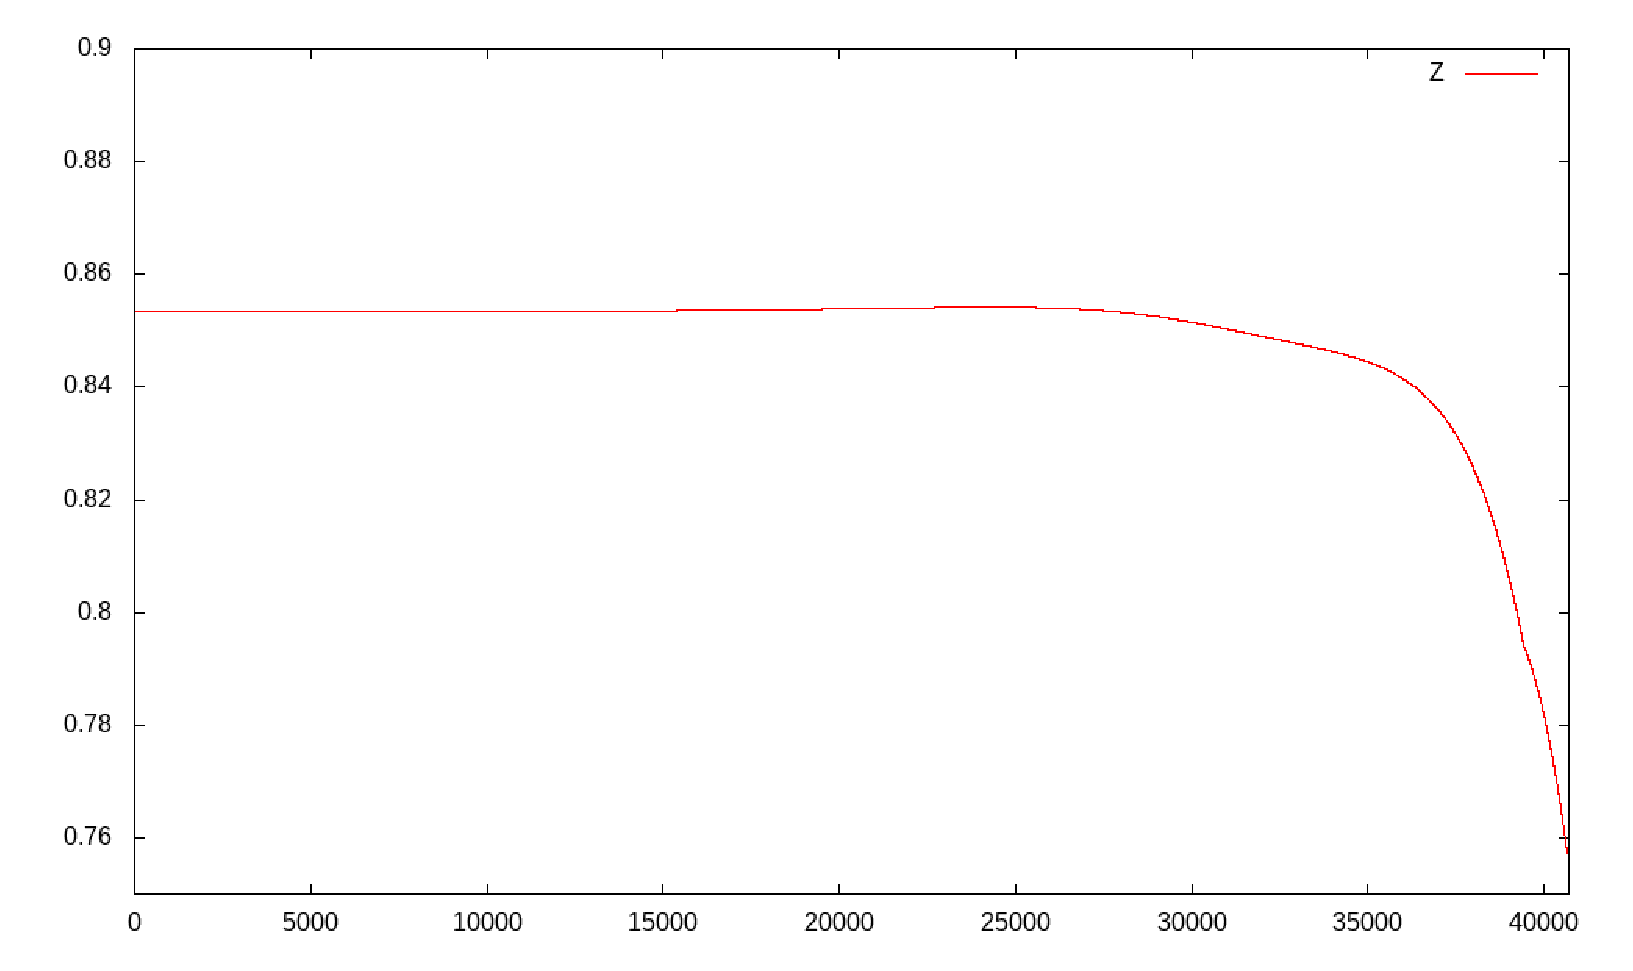
\includegraphics[scale=0.6]{Zeps}
\caption{Зависимость автокорреляционной функции скорости частиц от шага по времени.}
\end{figure}

\subsection{Контроль температуры}
Также в программе требовалось реализовать контроль температуры системы, суть которого заключается в том, чтобы, после некоторого шага моделирования, когда система придёт к положению равновесия при температуре $T_{current}$, сообщить системе некий импульс путем умножения скоростей всех частиц системы на коэффициент $\sqrt{{T_{desired}}/{T_{current}}}$, где $T_{desired}$ - требуемая температура системы, которой той необходимо достичь.
\

На рисунках 1.9 и 1.10 представлены характерные зависимости кинетической, потенциальной, полной энергий системы от шага по времени, а также температуры и средней температуры системы от шага по времени при реализованном контроле температуры.

\

Из зависимости энергии системы от шага по времени (рисунок 1.9) при реализованном контроле температуры видно, что и после релаксации системы к заданной температуре закон сохранения энергии продолжает выполняться, хотя полная энергия также релаксировала к другому значению.

\begin{figure}[!h]
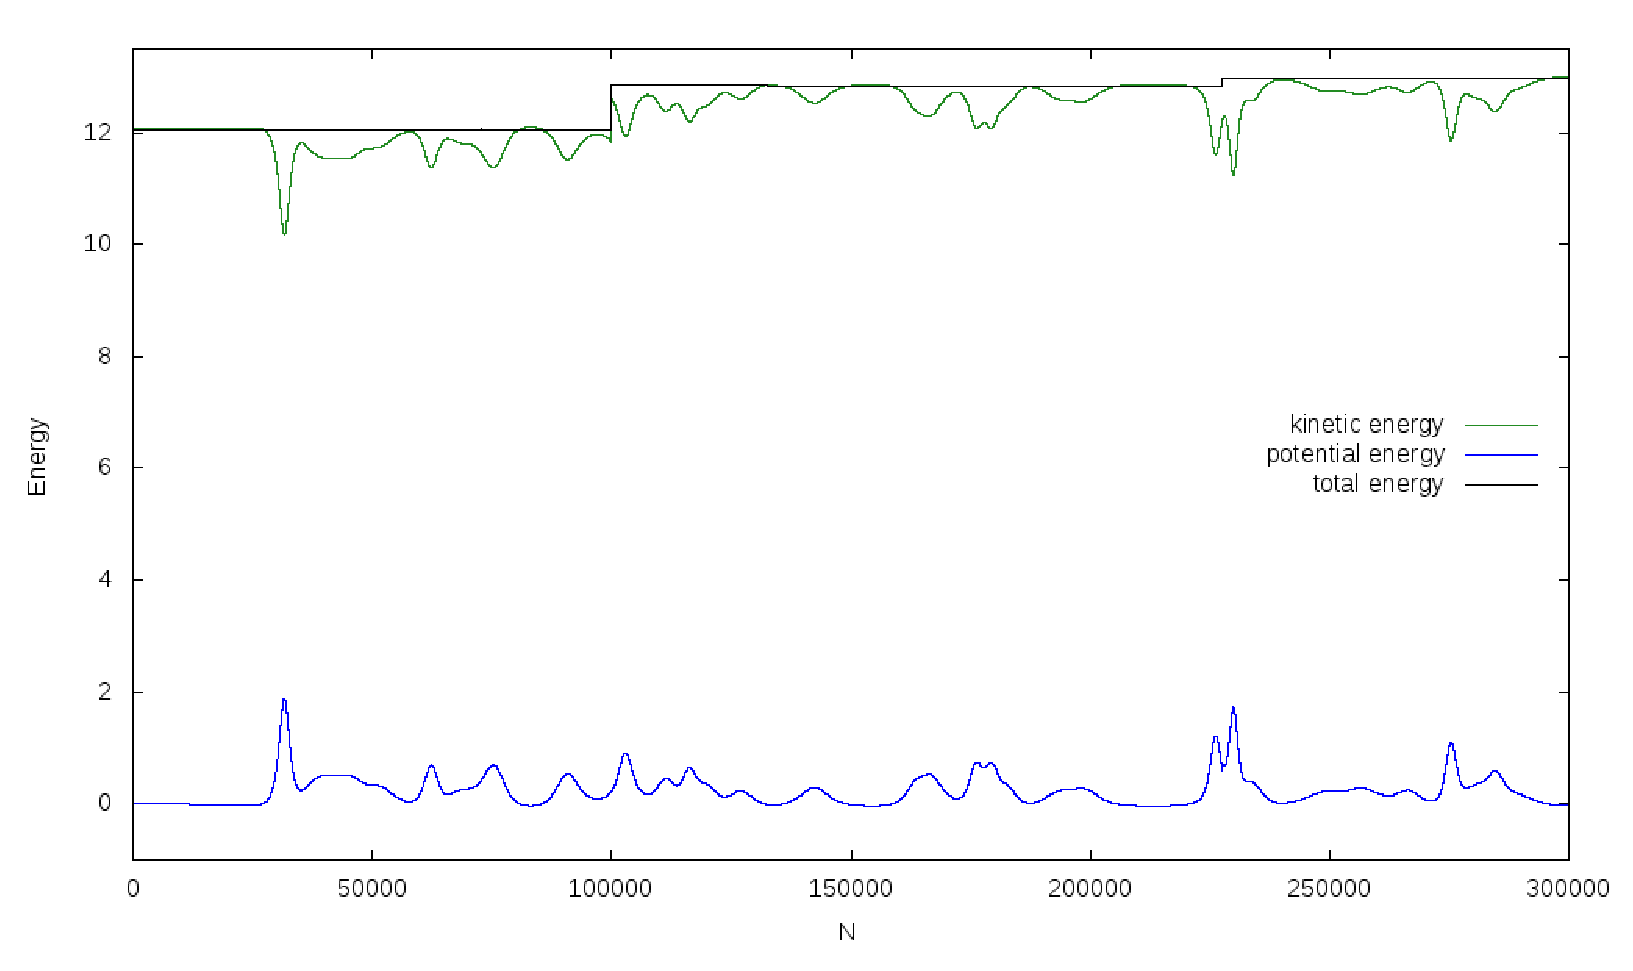
\includegraphics[scale=0.6]{energy300}
\caption{Зависимость средней (зеленый) и мгновенной (красный) температуры системы от шага по времени при реализованном контроле температуры.}
\end{figure}
\begin{figure}[!h]
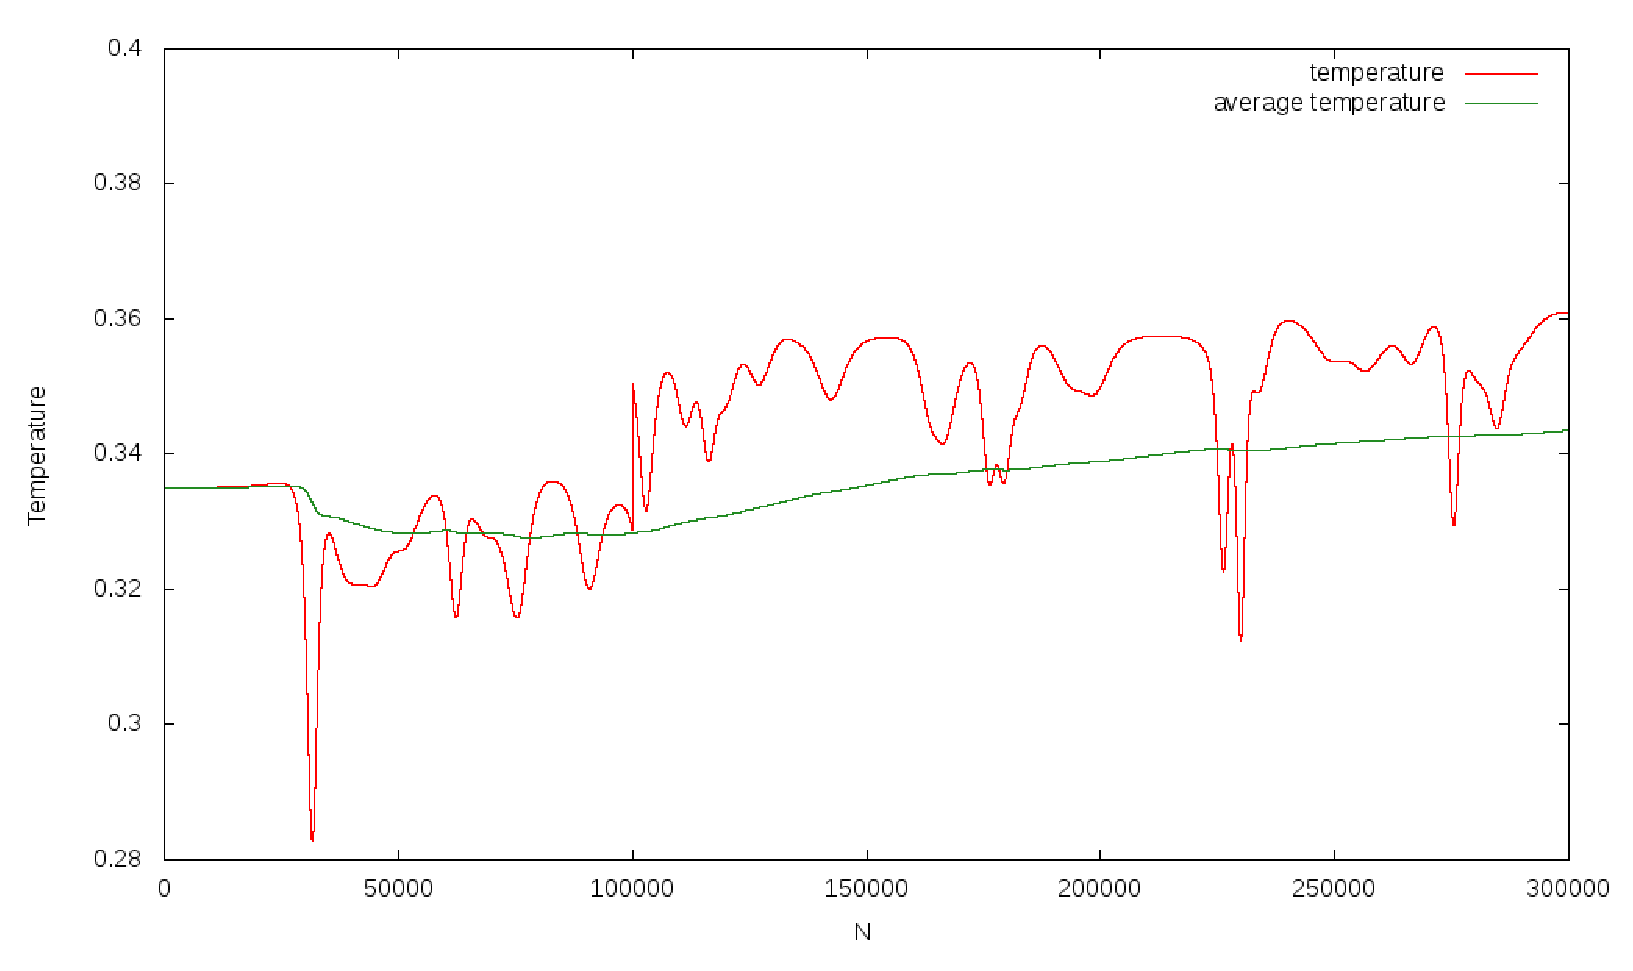
\includegraphics[scale=0.6]{temp300}
\caption{Зависимость средней (зеленый) и мгновенной (красный) температуры системы от шага по времени при реализованном контроле температуры.}
\end{figure}
\

\newpage\section{Выводы}
В ходе выполнения работы была разработана программа для моделирования двумерной системы частиц, взаимодействующих через потенциал Леннарда-Джонса. Была реализована возможность задания произвольного числа частиц, расчёт кинетической, потенциальной и полной энергий системы, определение и контроль температуры, визуализация всей системы и траектории отдельной её частицы, а также расчёт среднеквадратичного смещения и автокорреляционной функции скорости. В результате моделирования были получены и проанализированы все соответствующие графики зависимостей величин от времени, из которых можно получать информацию о характере движения частиц в системе и оценить правильность реализованного моделирования системы. Запуск программы при различных входных данных, согласующихся с физическими представлениями о динамике многочастичных систем, показал, что моделирование системы происходит корректно.
\end{document}
